\chapter{Course Introduction}
\label{cha:intro}

\sloppy
%\lecture{1 --- Wednesday, February 19th}
%{Spring 2020}{Rasmus Kyng}{Course Introduction}

\section{Overview}
 This course will take us quite deep into modern approaches to
 graph algorithms using convex optimization techniques.
%
 By studying convex optimization through the lens of graph algorithms,
 we'll try to develop an understanding of fundamental
 phenomena in optimization.
 %
 Much of our time will be devoted to flow problems on graphs.
 We will not only be studying these problems for their own sake,
 but also because they often provide a useful setting for thinking more broadly about optimization.

 The course will cover some traditional discrete approaches to various graph
 problems, especially flow problems, and then contrast these approaches
 with modern, asymptotically faster methods based on combining convex
 optimization with spectral and combinatorial graph theory.

\section{Electrical Flows and Voltages - a Graph Problem from Middle School?}

We will dive right into graph problems by considering how electrical
current moves through a network of resistors.

First, let us recall some middle school physics.
If some of these things don't make sense to you, don't worry, in less
than a paragraph from here, we'll be back to safely doing math.

Recall that a typical battery that one buys from Migros has two
endpoints, and produces what is called a \emph{voltage
  difference} between these endpoints.

One end of the battery will have a positive charge (I think that means an excess of
positrons\footnote{I'm joking, of course! Try Wikipedia if you want to know
more. However, you will not need it for this class.}), and the other a
negative charge.
If we connect the two endpoints with a wire, then a current will flow
from one end of the battery to the other in an attempt to even out
this imbalance of charge.

\begin{figure}[H]
  \centering
  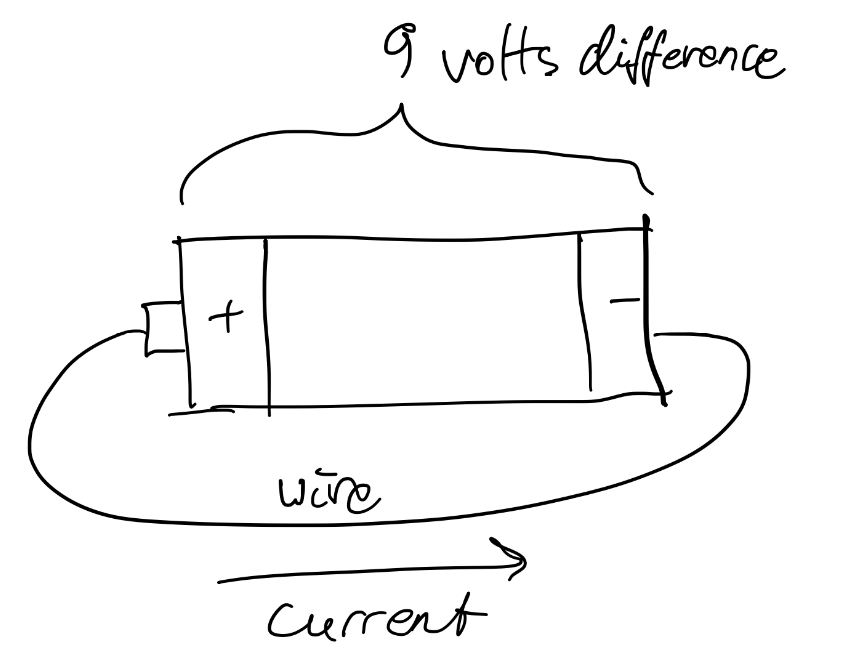
\includegraphics[width=0.5\linewidth]{fig/lecture1_battery9volts.png}
  \captionof{figure}{A 9 volts battery with a wire attached.}
  \label{fig:battery-volt}
\end{figure}

We can also imagine a kind of battery that tries to send a certain
amount of current through the wires between its endpoints, e.g. 1 unit of charge per
unit of time.
This will be a little more convenient to work with, so let us focus on
that case.

\begin{figure}[H]
  \centering
  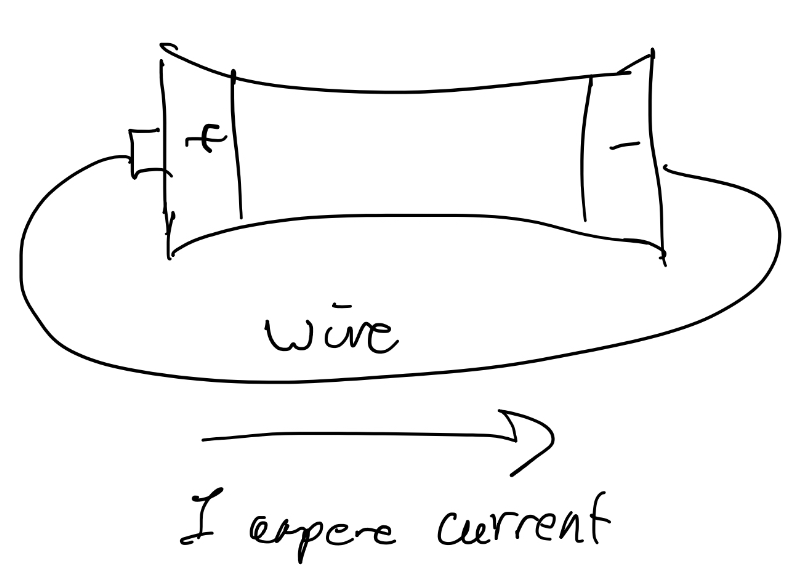
\includegraphics[width=0.5\linewidth]{fig/lecture1_battery1ampere.png}
  \captionof{figure}{A 1 ampere battery with a wire attached.}
  \label{fig:battery-current}
\end{figure}

A \emph{resistor} is a piece of wire that connects two
points $u$ and $v$, and is completely described by a single number $r$
called its \emph{resistance}.

If the voltage difference between the endpoints of the resistor is
$x$, and the resistance is $r$ then this will create a flow of charge per unit of time of $f = x / r$.
This is called Ohm's Law.

\begin{figure}[H]
  \centering
  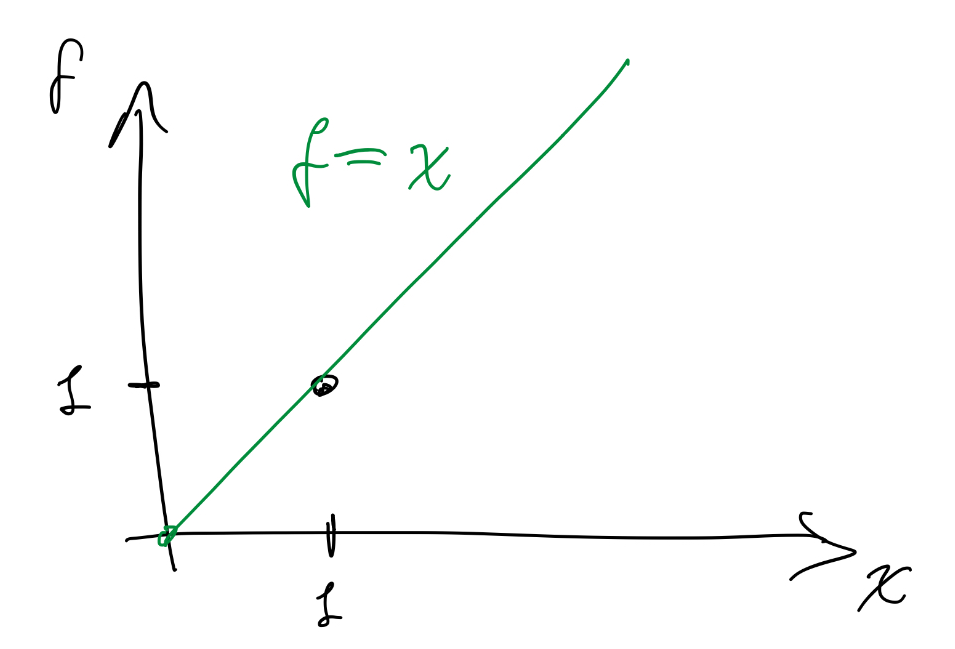
\includegraphics[width=0.5\linewidth]{fig/lecture1_ohmslawx-vs-f.png}
  \captionof{figure}{Ohm's Law for a resistor with resistance $r = 1$.}
  \label{fig:ohmslaw}
\end{figure}

Suppose we set up a bunch of wires that route electricity from our
current source $s$ to our current sink $t$ in some pattern:

\begin{figure}[H]
  \centering
  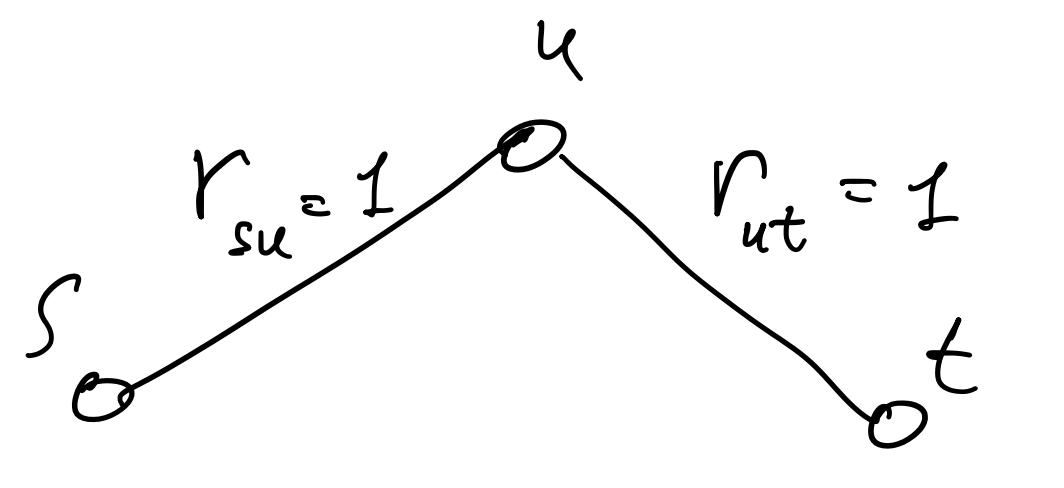
\includegraphics[width=0.5\linewidth]{fig/lecture1_graphpath.png}
  \captionof{figure}{A path of two resistors.}
  \label{fig:graphpath}
\end{figure}

We have one unit of charge flowing out of $s$ per unit of time, and
one unit coming into $t$.
Because charge is conserved, the current flowing into any other point
$u$ must equal the amount flowing out of it.
This is called Kirchhoff's Current Law.

To send one unit of current from $s$ to $t$, we must be sending it
first from $s$ to $u$ and then from $u$ to $t$.
So the current on edge $(s,u)$ is 1 and the current on $(u,t)$ is 1.
By Ohm's Law, the voltage difference must also be 1 across each of the two
wires.
Thus, if the voltage is $x$ at $s$, it must be $x+1$ at $u$ and $x+2$
at $t$. What is $x$? It turns out it doesn't matter: We only care
about the differences. So let us set $x = 0$.

\begin{figure}[H]
  \centering
  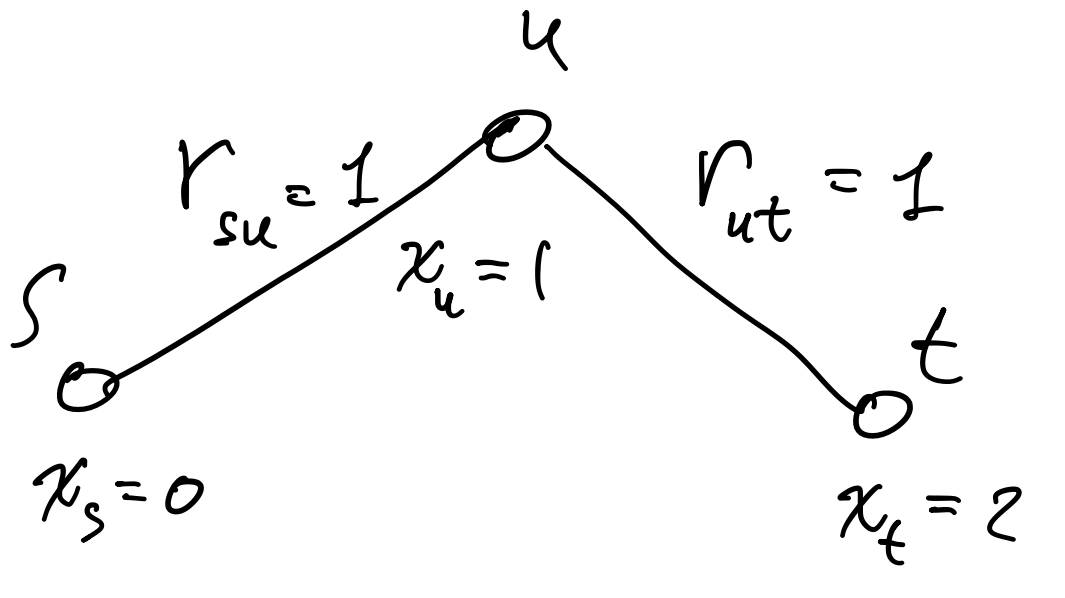
\includegraphics[width=0.5\linewidth]{fig/lecture1_graphpath-labelled.png}
  \captionof{figure}{A path of two resistors.}
  \label{fig:graphpathlabelled}
\end{figure}


Let us try one more example:

\begin{figure}[H]
  \centering
  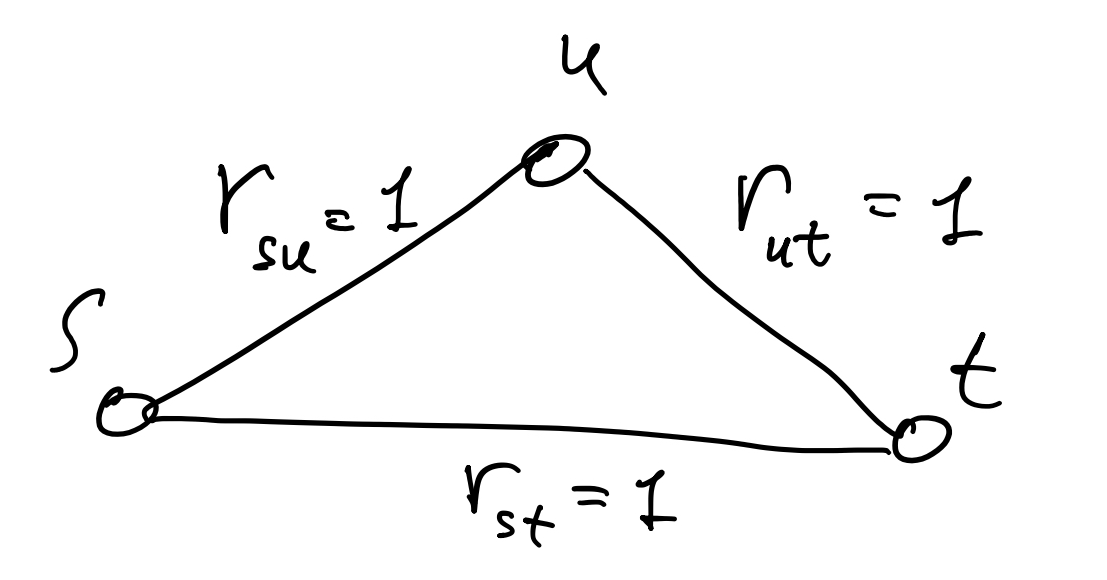
\includegraphics[width=0.5\linewidth]{fig/lecture1_graphtriangle.png}
  \captionof{figure}{A network with three resistors.}
  \label{fig:graphtriangle}
\end{figure}

How much flow will go directly from $s$ to $t$ and how much via $u$?

Well, we know what the net current flowing into and out of each vertex
must be, and we can use that to set up some equations.
Let us say the voltage at $s$ is $x_s$, at $u$ is $x_u$ and at $t$ is $x_t$.
\begin{tight_itemize}
\item Net current at $s$:   $-1 = (x_s-x_t) + (x_s-x_u)$
\item  Net current at $u$:   $\phantom{-}0 = (x_u-x_s) + (x_u-x_t)$
\item Net current at  $t$:\,   $\phantom{-}1 = (x_t-x_s)+(x_t-x_u)$
\end{tight_itemize}
The following is a solution: $x_s = 0$, $x_u = \frac{1}{3}$, $x_t
= \frac{2}{3}$.
And as before, we can shift all the voltages by some constant $x$ and
get another solution $x_s = x+0$, $x_u = x+\frac{1}{3}$, $x_t
= x+\frac{2}{3}$. You might want to convince yourself that these are the only solutions.

\paragraph{Electrical flows in general graphs.}
Do we know enough to calculate the electrical flow in some other
network of resistors?
To answer this, let us think about the network
as a graph.
Consider an undirected graph $G = (V,E)$ with $\abs{V} = n$ vertices and
$\abs{E} = m$ edges, and let us assume $G$ is connected.
Let's associate a resistance
$\rr(e) > 0$ with every edge $e \in E$.

To keep track of the direction of the flow on each edge, it will be
useful to assign an arbitrary direction to every edge. So let's do
that, but remember that this is just a bookkeeping tool that helps
us track where flow is going.

A \emph{flow} in the graph is a vector $\ff: \R^E$.
%
The \emph{net flow} of $\ff$ at a vertex $u \in V$ is defined as
$\sum_{v \to u} \ff(v,u) - \sum_{u  \to v} \ff(u,v).$
% As a second accounting trick, we can define $\ff(v,u) \defeq
% -\ff(u,v)$,
% and then write the net flow as $\sum_{(u,v)\in E} \ff(u,v)$.

We say a flow routes the demands $\dd \in \R^V$ if the net flow at
every vertex $v$ is $\dd(v)$.

We can assign a voltage to every vertex $\xx \in R^V$.
Ohm's Law says that the electrical flow induced by these voltages will
be $\ff(u,v) = \frac{1}{\rr(u,v)} (\xx(v) - \xx(u))$.

Say we want to route one unit of current from vertex $s \in V$ to vertex
$t \in V$.
As before, we can write an equation for every vertex saying that the
voltage differences must produce the desired net current:
\begin{tight_itemize}
\item Net current at $s$:
  $\phantom{----,,,}-1 = \sum_{(s,v)} \frac{1}{\rr(s,v)} (\xx(v) - \xx(s))$
\item Net current at $u \in V\setminus\setof{s,t}$:
  $\phantom{..} 0 = \sum_{(u,v)} \frac{1}{\rr(u,v)} (\xx(v) - \xx(u))$
\item Net current at  $t$:  $\phantom{------,} 1=\sum_{(t,v)} \frac{1}{\rr(t,v)} (\xx(v) - \xx(t))$
\end{tight_itemize}
This gives us $n$ constraints, exactly as many as we have voltage
variables.
However we have to be a little careful when trying to conclude that a
solution exists, yielding voltages $\xx$ that gives induce an
electrical flow routing the desired demand.


You will prove in the exercises (Week 1, Exercise 3) that a solution $\xx$ exists. The proof requires two
important observations: Firstly that the graph is connected, and
secondly that summed over all vertices, the net demand is zero,
i.e. as much flow is coming into the network as is leaving it.

\paragraph{The incidence matrix and the Laplacian matrix.}
To have a more compact notation for net flow constraints, we also
introduce the \emph{edge-vertex incidence matrix} of the graph,
$\BB \in \R^{V \times E}$.
\[
  \BB(v,e) =
  \begin{cases}
    1 & \text{ if } e = (u,v) \\
    -1 &\text{ if } e = (v,u) \\
    0 &\text{ o.w.}
  \end{cases}
\]
%
Now we can express the net flow constraint that $\ff$ routes $\dd$ by
\[
  \BB \ff = \dd
  .
\]
This is also called a conservation constraint. In our examples so far,
we have $\dd(s) = -1$, $\dd(t) = 1$ and $\dd(u) = 0$ for all $u\in V\setminus\setof{s,t}$.

If we let $\RR = \diag_{e \in E} \rr(e)$
then Ohm's law tells us that $\ff = \RR^{-1}\BB^{\trp} \xx$.
Putting these observations together, we have $\BB \RR^{-1}\BB^{\trp}
\xx= \dd$.
The voltages $\xx$ that induce $\ff$ must solve this system of linear
equations, and we can use that to compute both $\xx$ and $\ff$.
It is exactly the same linear
equation as the one we considered earlier.
We can show that for a connected graph, a solution $\xx$
exists if and only if the
flow into the graph equals the net flow out, which we can express as
$\sum_{v} \dd(v) = 0$ or $\vecone^\trp \dd = 0$.
You will show this as part of Exercise 3.
This also implies that an electrical flow routing
$\dd$ exists if and only if the net
flow into the graph equals the net flow out, which we can express as
$\vecone^\trp \dd = 0$.


The matrix $\BB \RR^{-1}\BB^{\trp}$ is called the \emph{Laplacian} of
the graph and is usually denoted by $\LL$.

\paragraph{An optimization problem in disguise.}
So far, we have looked at electrical voltages and flows as arising
from a set of linear equations -- and it might not be apparent that
this has anything to do with optimization.
But transporting current through a resistor requires energy, which will be
dissipated as heat by the resistor (i.e. it will get hot!).
If we send a current of $f$ across a resistor with a potential drop of
$x$, then the amount of energy spent per unit of time by the resistor will be
$f \cdot x$. This is called Joule's Law.
Applying Ohm's law to a resistor with resistance $r$,
we can also express this energy per unit of time
as $f \cdot x = x^2 / r = r \cdot f ^2$.
Since we aren't bothering with units, we will even forget about time,
and refer to these quantities as ``energy'', even though a physicist
would call them ``power''.

\begin{figure}[H]
  \centering
  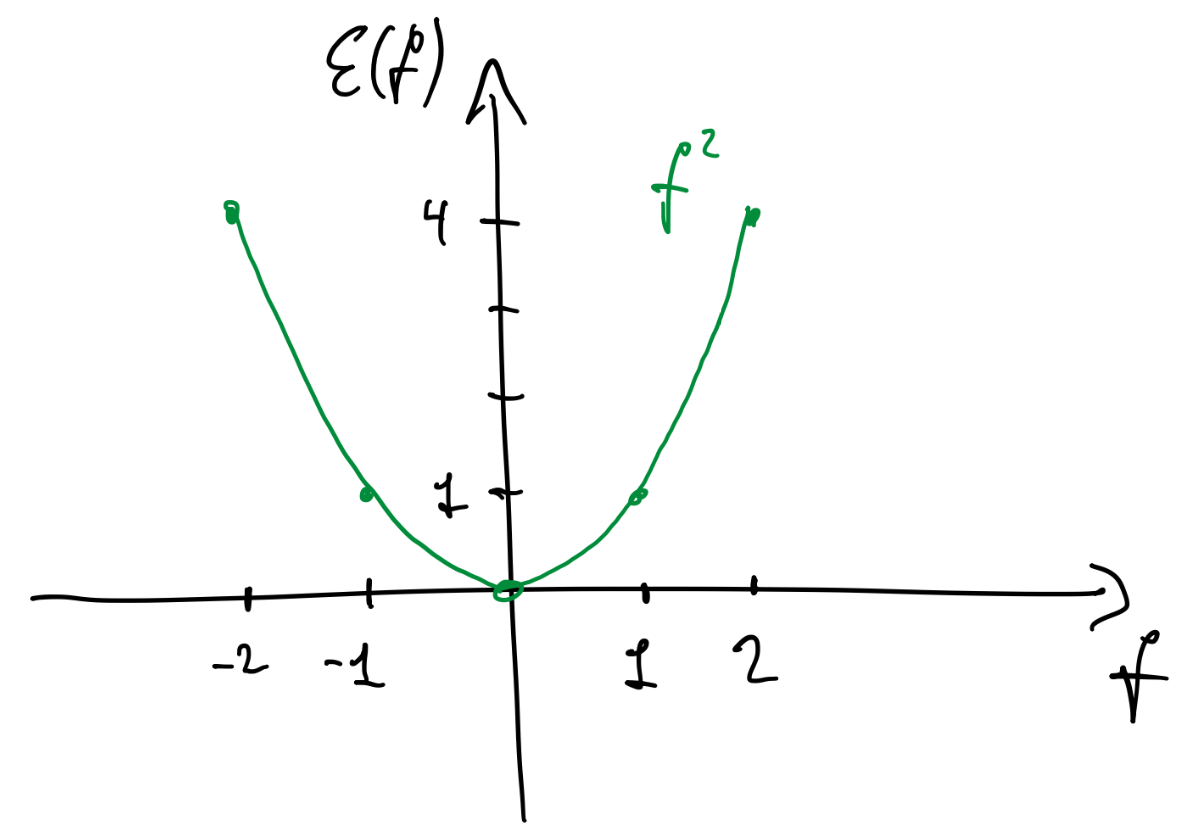
\includegraphics[width=0.6\linewidth]{fig/lecture1_flow-vs-energy.png}
  \captionof{figure}{Energy as a function of flow in a resistor with
    resistance $r = 1$.}
  \label{fig:flow-vs-energy}
\end{figure}

Now, another interesting question would seem to be: If we want to find
a flow routing a certain demand $\dd$, how should the flow behave in
order to minimize the electrical energy spent routing the flow?
The electrical energy of a flow vector $\ff$ is $\energy(\ff) \defeq \sum_e \rr(e) \ff(e)^2$.
We can phrase this as an optimization problem:
\begin{align*}
  \min_{\ff \in \R^E} \, & \energy(\ff)
  \\
  \textrm{s.t. } & \BB \ff = \dd .
\end{align*}
We call this problem \emph{electrical energy-minimizing flow}.
As we will prove later, the flow $\ff^*$ that minimizes the electrical
energy among all flows that satisfy $\BB \ff = \dd$ is precisely the
electrical flow.

\paragraph{A pair of problems.}
What about our voltages, can we also get them from some optimization
problem?
%
Well, we can work backwards from the fact that our voltages solve the
equation $\LL \xx = \dd$.
%
Consider the function $c(\xx) = \frac{1}{2} \xx^{\trp} \LL \xx -
\xx^{\trp}\dd$.
We should ask ourselves some questions about this function $c : \R^V
\to \R$. Is it continuous and continuously differentiable? The answer to this is
yes, and that is not hard to see.
Does the function have a minimum?
This is maybe not immediately clear, but the minimum does indeed exist.

When this is minimized, the derivative of $c(\xx)$ with respect to each coordinate of $\xx$
must be zero. This condition yields exactly the system of linear
equations $\LL \xx = \dd$.
You will confirm this in Exercise 4 of the first exercise sheet.

Based on our derivative condition for the optimum, we can also express the electrical voltages as the solution to
an optimization problem, namely
\begin{align*}
\min_{\xx \in \R^V} & c(\xx)
\end{align*}
As you are probably aware, having the derivative of each coordinate equal zero is not a
sufficient condition for being at the optimum of a
function\footnote{Consider the function in one variable $c(x) =
  x^3$.}.

It is also interesting to know whether \emph{all} solutions to $\LL
\xx = \dd$ are in fact minimizers of $c$. The answer is
yes, and we will see some very general tools for proving statements like
this in Chapter~\ref{sec:cvopt}.
% Although, we have not yet proven the electrical flow minimizes
% electrical energy $\sum_e \rr(e) \ff(e)^2$, I have promised you that
% this is true.
% Let us denote the electrical flow and voltages by $\fftil$ and $\xxtil$,
% and recall that $\fftil = \RR^{-1} \BB ^\trp \xxtil$.
% Based on this, we can make an interesting observation:
% \[
%   \sum_e \rr(e) \ff(e)^2
%   =
%   \ff^{\trp} \RR \ff
%   =
  % \]
  % \frac{1}{2} \xxtil^{\trp} \LL \xxtil - \xxtil^{\trp}\dd
  % =

Altogether, we can see that routing electrical current through a
network of resistors leads to a \emph{pair} of optimization problems,
let's call them $\ff^*$ and $\xx^*$,
and that the solutions to the two problems are related, in our case
through the equation $\ff^* = \RR^{-1}\BB^{\trp} \xx^*$ (Ohm's Law).
But why and how are these two optimization problems related?

Instead of minimizing $c(\xx)$, we can equivalently think about maximizing
$-c(\xx)$, which gives the following optimization problem: $\max_{\xx \in \R^V} -c(\xx)$.
In fact, as you will show in the exercises for Week 1,
we have $\energy(\ff^*) = -c(\xx^*)$, so the
minimum electrical energy is exactly the maximum value of
$-\cc(\xx)$.
More generally for \emph{any} flow that routes $\dd$ and \emph{any}
voltages $\xx$, we have $\energy(\ff) \geq -c(\xx)$.
So, for any $\xx$, the value of $-c(\xx)$ is a lower bound on the
minimum energy $\energy(\ff^*)$.

This turns out to be an instance of a much broader phenomenon, known
as Lagrangian duality, which allows us to learn a lot about many
optimization problems by studying two related pairs of problems, a
minimization problem, and a related maximization problem that gives
lower bounds on the optimal value of the minimization problem.

\paragraph{Solving $\LL \xx = \dd$.}
Given a graph $G$ with resistances for the edges, and some net flow
vector $\dd$, how quickly can we compute $\xx$?
%
Broadly speaking, there are two very different families of algorithms
we could use to try to solve this problem.

We could solve the linear equation using something like
\emph{Gaussian Elimination} to compute an exact solution.

Alternatively,
we could start with a guess at a solution, e.g. $\xx_0
= \veczero$, and then we could try to make a change to $\xx_0$ to reach
a new point $\xx_1$ with a lower value of $c(\xx) = \frac{1}{2} \xx^{\trp} \LL \xx -
\xx^{\trp}\dd$, i.e. $c(\xx_1) < c(\xx_0)$.
If we repeat a process like that for enough steps, say $t$, hopefully we
eventually reach $\xx_t$ with $c(\xx_t)$ close to $c(\xx^*)$, where
$\xx^*$ is a minimizer of $c(\xx)$ and hence $\LL \xx^* = \dd$.
Now, we also need to make sure that $c(\xx_t) \approx c(\xx^*)$
implies that $\LL \xx_t \approx \dd$ in some useful sense.

One of the most basic algorithms in this framework of ``guess and adjust''
is called \emph{Gradient Descent}, which we will study in Week 2.
The rough idea is the following: if we make a very small step from $\xx$ to
$\xx + \ddelta$, then a multivariate Taylor expansion suggests that
$c(\xx + \ddelta) - c(\xx) \approx \sum_{v \in V} \ddelta(v)
\frac{\partial c(\xx)}{\partial\xx(v)} $.

If we are dealing with smooth convex function,
this quantity is negative if we let $\ddelta(v) = -\epsilon \cdot \frac{\partial
  c(\xx)}{\partial\xx(v)}$ for some small enough $\epsilon$ so the
approximation holds well.
So we should be able to make progress by taking a small step in this
direction.
That's Gradient Descent!
The name comes from the vector of partial
derivatives, which is called the gradient.
% But first we need to become familiar with some basic terminology about
% optimization and some convex geometry.
% As we will see later in this course, understanding electrical problems
% from an optimization perspective is crucial to developing fast
% algorithms.

As we will see later in this course, understanding electrical problems
from an optimization perspective is crucial to develop fast
algorithms for computing electrical flows and voltages, but to do very
well, we also need to borrow some ideas from Gaussian Elimination.

What running times do different approaches get?
\begin{enumerate}
\item Using Gaussian Elimination, we can find $\xx$ s.t. $\LL \xx =
  \dd$ in $O(n^3)$ time and with asymptotically faster algorithms based on matrix
  multiplication, we can bring this down to roughly $O(n^{2.372})$.
\item Meanwhile Gradient Descent will get a running time of $O(n^3m)$
  or so -- at least this is a what a simple analysis suggests.
\item However, we can do much better: By combining ideas from both
  algorithms, and a bit more,
  we can get $\xx$ up to very high
  accuracy in time $O(m \log^c n)$ where $c$ is some small constant.
  % This type of result was orignally shown by Spielman and Teng in a
  % breakthrough result in 2004.
\end{enumerate}


\section{Convex Optimization}

Recall our plot in Figure~\ref{fig:flow-vs-energy} of the energy required to
route a flow $f$ across a resistor with resistance $r$, which was
$\energy(f) = r\cdot f^2$.
%
We see that the function has a special structure: the graph of the function sits
below the line joining any two points $(f, \energy(f))$ and $(g,\energy(g))$.
A function $\energy : \R \to \R$ that has this property is said to be convex.

Figure~\ref{fig:flow-vs-energy-convex} shows the energy as a function of flow, along with two
points $(f, \energy(f))$ and $(g,\energy(g))$. We see the function sits below the
line segment between these points.

\begin{figure}[H]
  \centering
  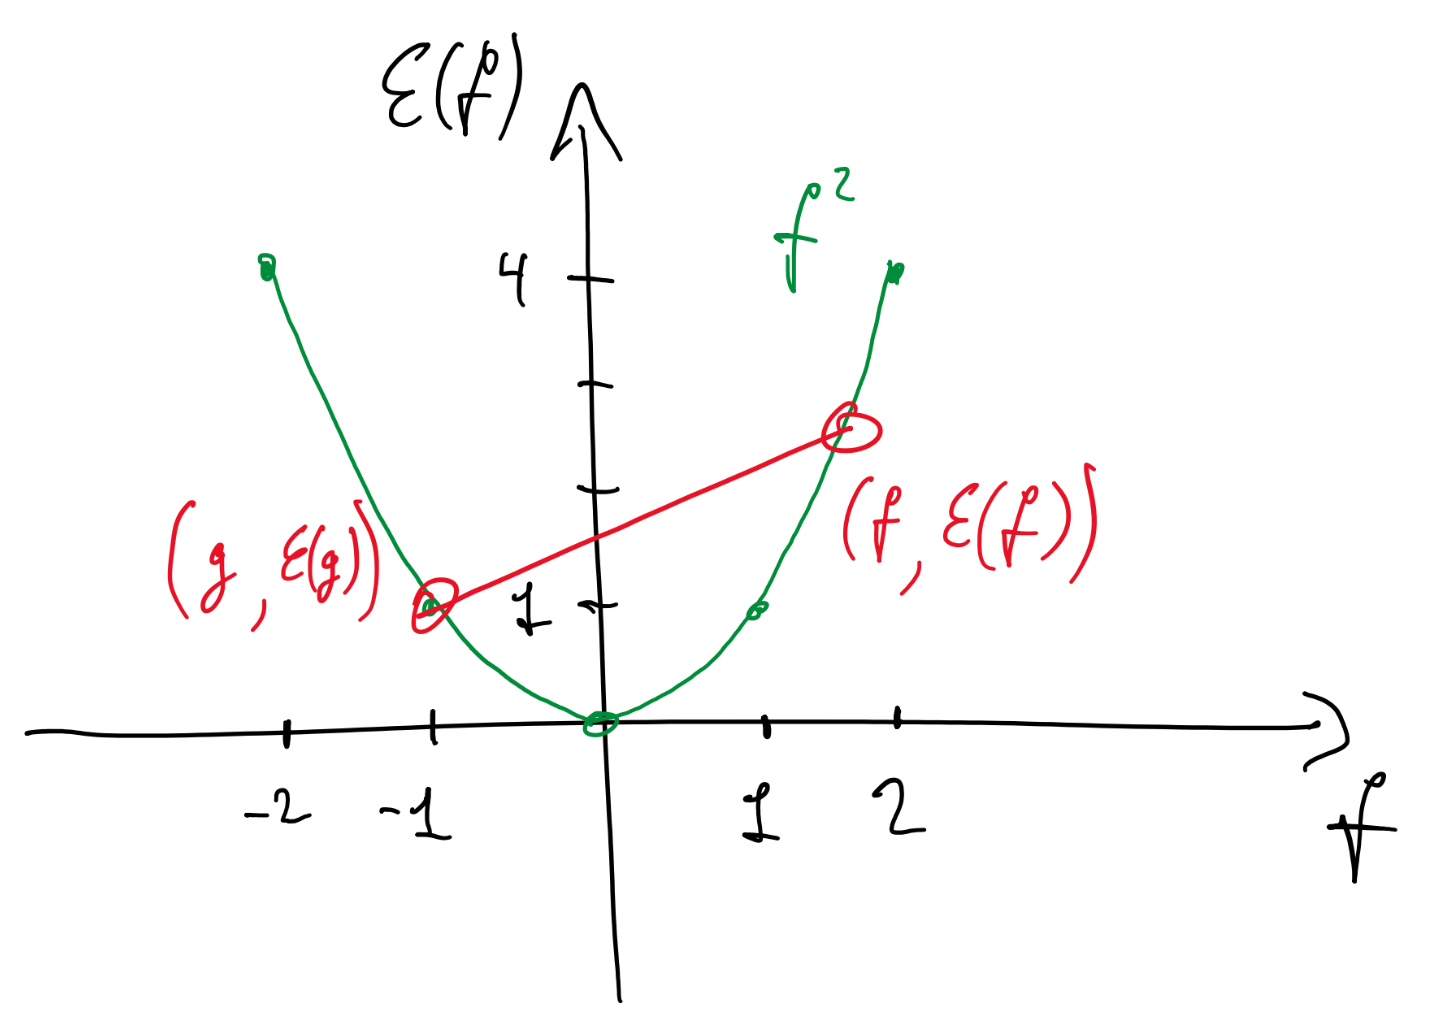
\includegraphics[width=0.6\linewidth]{fig/lecture1_flow-vs-energy-convex.png}
  \captionof{figure}{Energy as a function of flow in a resistor with
    resistance $r = 1$. The function is convex.}
  \label{fig:flow-vs-energy-convex}
\end{figure}
We can also interpret this condition as saying that for all $\theta \in [0,1]$
\[
  \energy(\theta f + (1-\theta)g) \leq \theta \energy(f) +
  (1-\theta) \energy(g)
  .
  \]
This immediately generalizes to functions $\energy:\R^m \to \R$.

A \emph{convex set} is a subset of $S \subseteq \R^m$ s.t.
if $\ff, \gg \in S$ then for all $\theta \in [0,1]$ we have
$\theta \ff + (1-\theta) \gg \in S$.

Figure~\ref{fig:convex_sets} shows some examples of sets that are and
aren't convex.

\begin{figure}[t]
\begin{centering}
                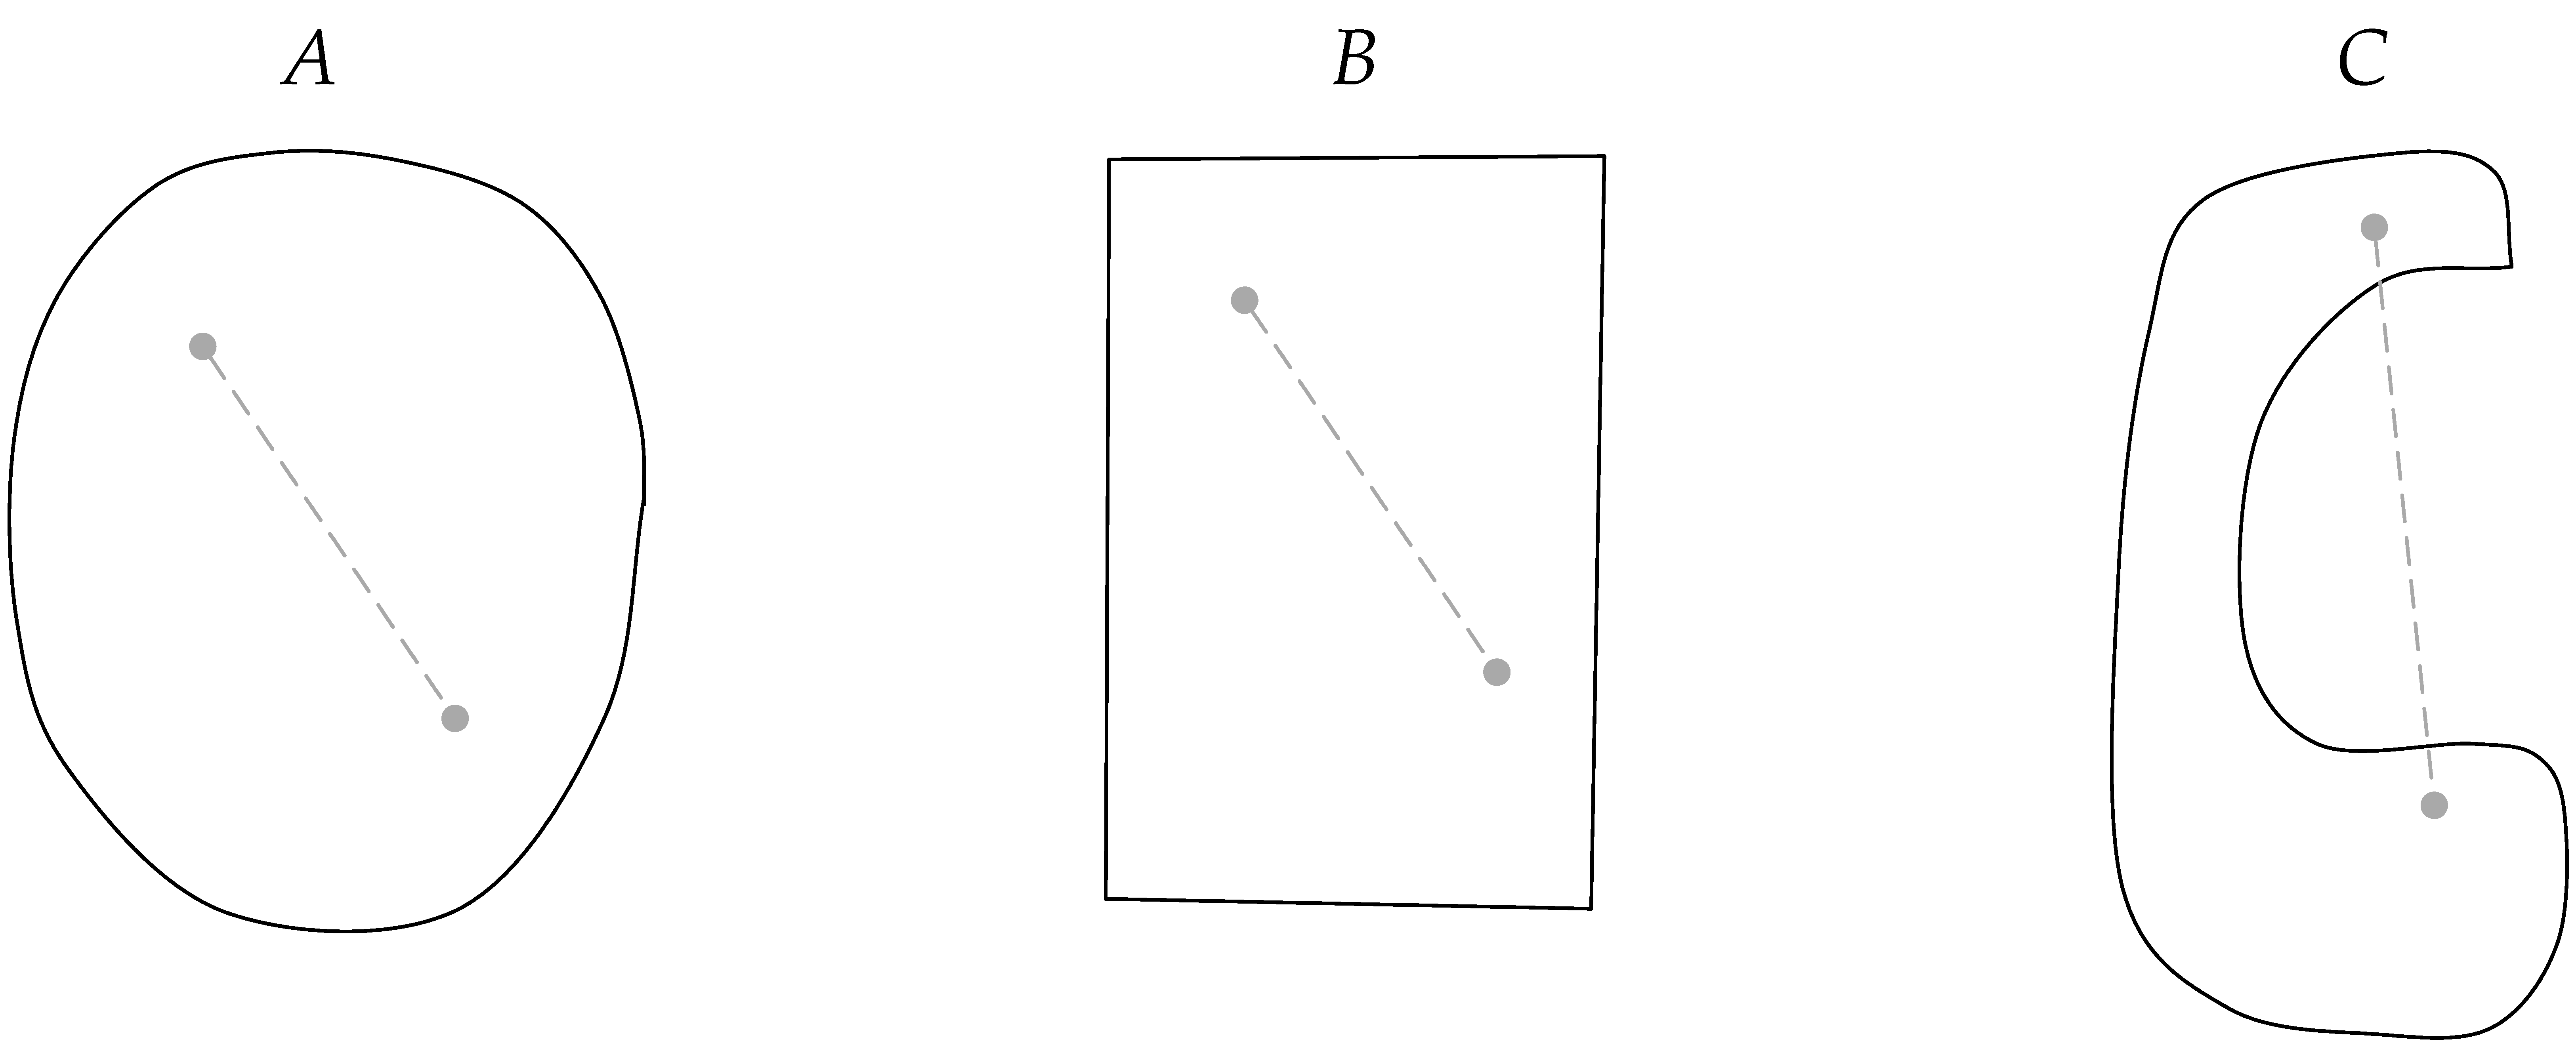
\includegraphics[trim = 0mm 0mm 0mm 0mm, height=60mm]{fig/lec1_convex_sets.pdf}
                 \caption{A depiction of convex and non-convex sets.  The sets $A$ and $B$ are convex since the straight line between any two points inside them is also in the set.  The set $C$ is not convex.}\label{fig:convex_sets}
                 \end{centering}
\end{figure}


Convex functions and convex sets are central to optimization,
because for most problems of minimization of a convex function over a
convex set, we can develop fast algorithms \footnote{
 There are some convex optimization problems that are NP-hard.
  That said, polynomial time algorithms exist for almost any convex
  problem you can come up with.
  The most general polynomial time algorithm for convex optimization
  is probably the
  \href{https://en.wikipedia.org/wiki/Ellipsoid_method}{Ellipsoid Method}.
}.


So why convex functions and convex sets?
One important reason is that
for a convex function defined over a convex feasible set,
any local minimum is also a global minimum,
and this fact makes searching for an optimal solution
computationally easier.
In fact, this is closely related to why Gradient Descent works well
on many convex functions.


Notice that the set $\setof{ \ff: \BB \ff = \dd}$ is convex, i.e. the
set of all flows that route a fixed demand $\dd$ is convex.
It is also easy to verify that $\energy(\ff) = \sum_e \rr(e) \ff(e)^2$
is a convex function, and hence finding an electrical flow is an
instance of convex minmization:



\section{More Graph Optimization Problems}

\paragraph{Maximum flow.}
Again, let $G=(V,E)$ be an undirected, connected graph with $n$
vertices and $m$ edges.
Suppose we want to find a flow
$\ff \in \R^E$ that routes $\dd$, but instead of trying to minimize
electrical energy, we try to pick an $\ff$ that minimizes the largest
amount of flow on any edge, i.e. $\max_e \abs{\ff_e}$  -- which we
also denote by $\norm{\ff}_{\infty}$.
We can write this problem as
\begin{align*}
\min_{\ff \in \R^E } & \norm{\ff}_{\infty} \\
\textrm{s.t. } & \BB \ff = \dd
\end{align*}
This problem is known as the Minimum Congested Flow Problem\footnote{This
  version is called undirected, because the graph is undirected, and
  \emph{uncapacitated} because we are aiming for the same
  bound on the flow on all edges.}.
It is equivalent to the more famous Maximum Flow Problem.

The behavior of this kind of flow is very different than electrical
flow. Consider the question of whether a certain demand can be routed
$\norm{\ff}_{\infty} \leq 1$.
Imagine sending goods from a source $s$ to a destination $t$ using a
network of train lines that all have the
same capacity and asking whether the network is able to route the
goods at the rate you want: This boils down to whether routing exists
with $\norm{\ff}_{\infty} \leq 1$, if we set it up right.

We have a very fast, convex optimization-based algorithm for Minimum Congested Flow:
In $m \epsilon^{-1} \log^{O(1)} n$ time, we can find a flow $\fftil$
s.t. $\BB \fftil = \dd$ and $\norm{\fftil}_{\infty} \leq
(1+\epsilon)\norm{\ff^*}_{\infty}$, where $\ff^*$ is an optimal solution, i.e. an
actual minimum congestion flow routing $\dd$.

But what if we want $\epsilon$ to be very small, e.g. $1/m$? Then this running
time isn't so good anymore.
But, in this case, we can use other algorithms that find flow $\ff^*$
\emph{exactly}. Unfortunately, these algorithms take time roughly $m^{4/3+o(1)}$.

Just as the electrical flow problem had a dual voltage problem, so
maximum flow has a dual voltage problem, which is know as the
$s$-$t$ minimum cut problem.

\paragraph{Maximum flow, with directions and capacities.}
We can make the maximum flow problem harder by introducing directed
edges: To do so, we allow edges to exist in both directions between vertices, and we require that the flow on a directed edge is
always non-negative. So now $G=(V,E)$ is a directed graph.
We can also make the problem harder by introducing capacities.
We define a capacity vector $\cc \in \R^E \geq \veczero$ and try to minimize $\norm{\CC^{-1} \ff}_{\infty}$, where $\CC =
\diag_{e \in E}\cc(e)$.
Then our problem becomes
\begin{align*}
\min_{\ff \in \R^E } & \norm{\CC^{-1} \ff}_{\infty} \\
  \textrm{s.t. } &  \BB \ff = \dd\\
                     &  \ff \geq \veczero.
\end{align*}
For this capacitated, directed maximum flow problem, our best
algorithms run in about $O( m \sqrt{n} )$ time in sparse graphs and $O(
m^{1.483} )$ in dense graphs\footnote{Provided the
  capacities are integers satisfying a condition like $\cc \leq n^{100} \vecone$.}, even if we are willing to
accept fairly low accuracy solution.
If the capacities are allowed to be exponentially large, the best
running time we can get is $O(m n)$.
For this problem, we do not yet know how to improve over classical
combinatorial algorithms using convex optimization.

\paragraph{Multi-commodity flow.}
We can make the problem even harder still, by simultaneously trying to route
two types of flow (imagine pipes with Coke and Pepsi).
Our problem now looks like
\begin{align*}
\min_{\ff_1, \ff_2 \in \R^E } & \norm{\CC^{-1} (\ff_1 + \ff_2)}_{\infty} \\
  \textrm{s.t. } &  \BB \ff_1 = \dd_1 \\
                              & \BB \ff_2 = \dd_2\\
                     &  \ff_1, \ff_2 \geq \veczero.
\end{align*}
Solving this problem to high accuracy is essentially as hard as
solving a general linear program! We should see later in the course
how to make this statement precise.

If we in the above problem additionally require that our flows must be
integer valued, i.e. $\ff_1, \ff_2 \in \N_{0}$, then the problem becomes NP-complete.

\paragraph{Random walks in a graph.}
Google famously uses\footnote{At least they did at some point.} the
PageRank problem to help decide how to rank their search results.
This problem essentially boils down to computing the \emph{stable
distribution} of a random walk on a graph.
Suppose $G=(V,E)$ is a directed graph where each outgoing edge
$(v,u)$, which we will define as going from $u$ to $v$, has a
transition probability $p_{(v,u)} > 0$ s.t. $\sum_{z \leftarrow u}
p_{(z,u)} = 1$.
We can take a step of a random walk on the vertex set by starting at some vertex
$u_0 = u$, and then randomly pick one of the outgoing edges
$(v,u)$ with probability $p_{(v,u)}$  and move to
the chosen vertex $u_1 = v$.  Repeating this procedure, to take a step from
the next vertex $u_1$, gives us a
\emph{random walk} in the graph, a sequence of vertices $u_0, u_1, u_2
\ldots, u_k$.

We let $\PP \in \R^{V \times V}$ be the matrix of transition
probabilities given by
\[
  \PP_{vu} =
  \begin{cases}
    p_{(v,u)} & \text{ for } (u,v) \in E \\
    0 & \text{ o.w.}
  \end{cases}
\]

Any probability distribution over the vertices can be specified by a vector
$\pp \in \R^V$ where $\pp \geq
\veczero$ and $\sum_v \pp(v) = 1$.
We say that probability distribution $\ppi$ on the vertices is a \emph{stable distribution} of the random walk
if $\ppi = \PP \ppi$.
A strongly connected graph always has exactly one stable distribution.

How quickly can we compute the stable distribution of a general random
walk? Under some mild conditions on the stable
distribution\footnote{Roughly something like $\max_{v} 1/\ppi(v) \leq n^{100}$.}, we can find
a high accuracy approximation of $\ppi$ in time $O(m \log^cn )$ for
some constant $c$.

This problem does not easily fit in a framework of convex
optimization, but nonetheless, our fastest algorithms for it use ideas
from convex optimization.

\section*{Topics in this Course}
In this course, we will try to address the following questions.
\begin{enumerate}
\item What are the fundamental tools of fast convex optimization?
\item What are some problems we can solve quickly on graphs using optimization?
\item What can graphs teach us about convex optimization?
\item What algorithm design techniques are good for getting algorithms
  that quickly find a crude approximate solution? And what techniques
  are best when we need to get a highly accurate answer?
\item What is special about flow problems?
\end{enumerate}



%%% Local Variables:
%%% mode: latex
%%% TeX-master: "main"
%%% TeX-engine: luatex
%%% End:
